\label{research}
So far, we discussed an extension of the pilot abstraction to support data analytics and task based data intensive applications on HPC resources, a comparison between different task-based data oriented frameworks, and a design comparison for scientific workflows.
In addition, we identified a need for the execution of scientific computational campaigns with minimum user intervention, independent from users' scientific domain.
In this section, we motivate and propose a Campaign Manager (CM) for creating and enacting a campaign execution plan. \mtnote{Do we need to explain how these three topics fit together?}


\subsection{Proposed Topic}
%Campaigns from the biomolecular and earth sciences are diverse in terms of composition, number and size of workflow members, and dynamicity. \mtnote{What does ``composition'' stand for in this context?}
%Biomolecular science campaigns may be comprised of a small number of workflows with millions of tasks, or thousands of workflows with tens to hundreds tasks~\cite{dakka2018high}. \mtnote{And everything in between these two boundaries?}
%Earth sciences campaigns, especially those which use VHR \mtnote{expand if not used before} satellite imagery, comprise of workflows with thousands of tasks.
%The number of workflows depends on the number of images the user has access to as well as the time they are able to obtain imagery.
%These workflows can be static~\cite{paraskevakos2019workflow} or dynamic~\cite{dakka2018high}. \mtnote{Did we explained why campaigns from these two science domains are interesting for this proposal?}

% ------------------------------------------------------------------------------
% Scientific campaigns
Scientific campaigns execute workflows on heterogeneous resources either for large periods of time~\cite{maeno2008panda} or with a given objective.
This objective can be translated to a computational objective function that would either minimize or maximize a computational metric.
Calculating the makespan of the campaign means finding the execution plan that satisfies the computational objective function.
%As a result, calculating the makespan of the campaign for based on workflow grouping, execution order, and workflow to resource mapping becomes important.
%The combination of workflow grouping, execution order, and workflow to resource mapping that produces a makespan which satisfies the computational objective of the campaign defines the execution plan of the campaign.


%Scientific workflows are generally described by direct acyclic graphs (DAG), where the nodes are tasks and the edges are dependencies.
%A subset of this general description of workflows are those which can be represented via the Pipeline, Stage, Task (PST) model~\cite{balasubramanian2018harnessing}. \mtnote{As discussed, EnTK and PST are implementation details.}
%The PST model describes workflows as a set of pipelines, where each pipeline is a sequence of stages.
%Each stage then is a set of tasks that need to be executed.
%Concurrency is achieved at the level of pipelines and the level of tasks. 
%Based on our use cases, we are particularly interested in scientific campaigns comprised by workflows that can be described via the PST model. \mtnote{Why?}
%Figure~\ref{fig:bio_earth_workflows} shows two example workflows from the biomolecular sciences (Fig.~\ref{fig:bio_workflow}) and the earth sciences (Fig.~\ref{fig:earth_workflow}). 

%\begin{figure*}[ht!]
%    \centering
%    \begin{subfigure}[b]{0.45\textwidth}
%         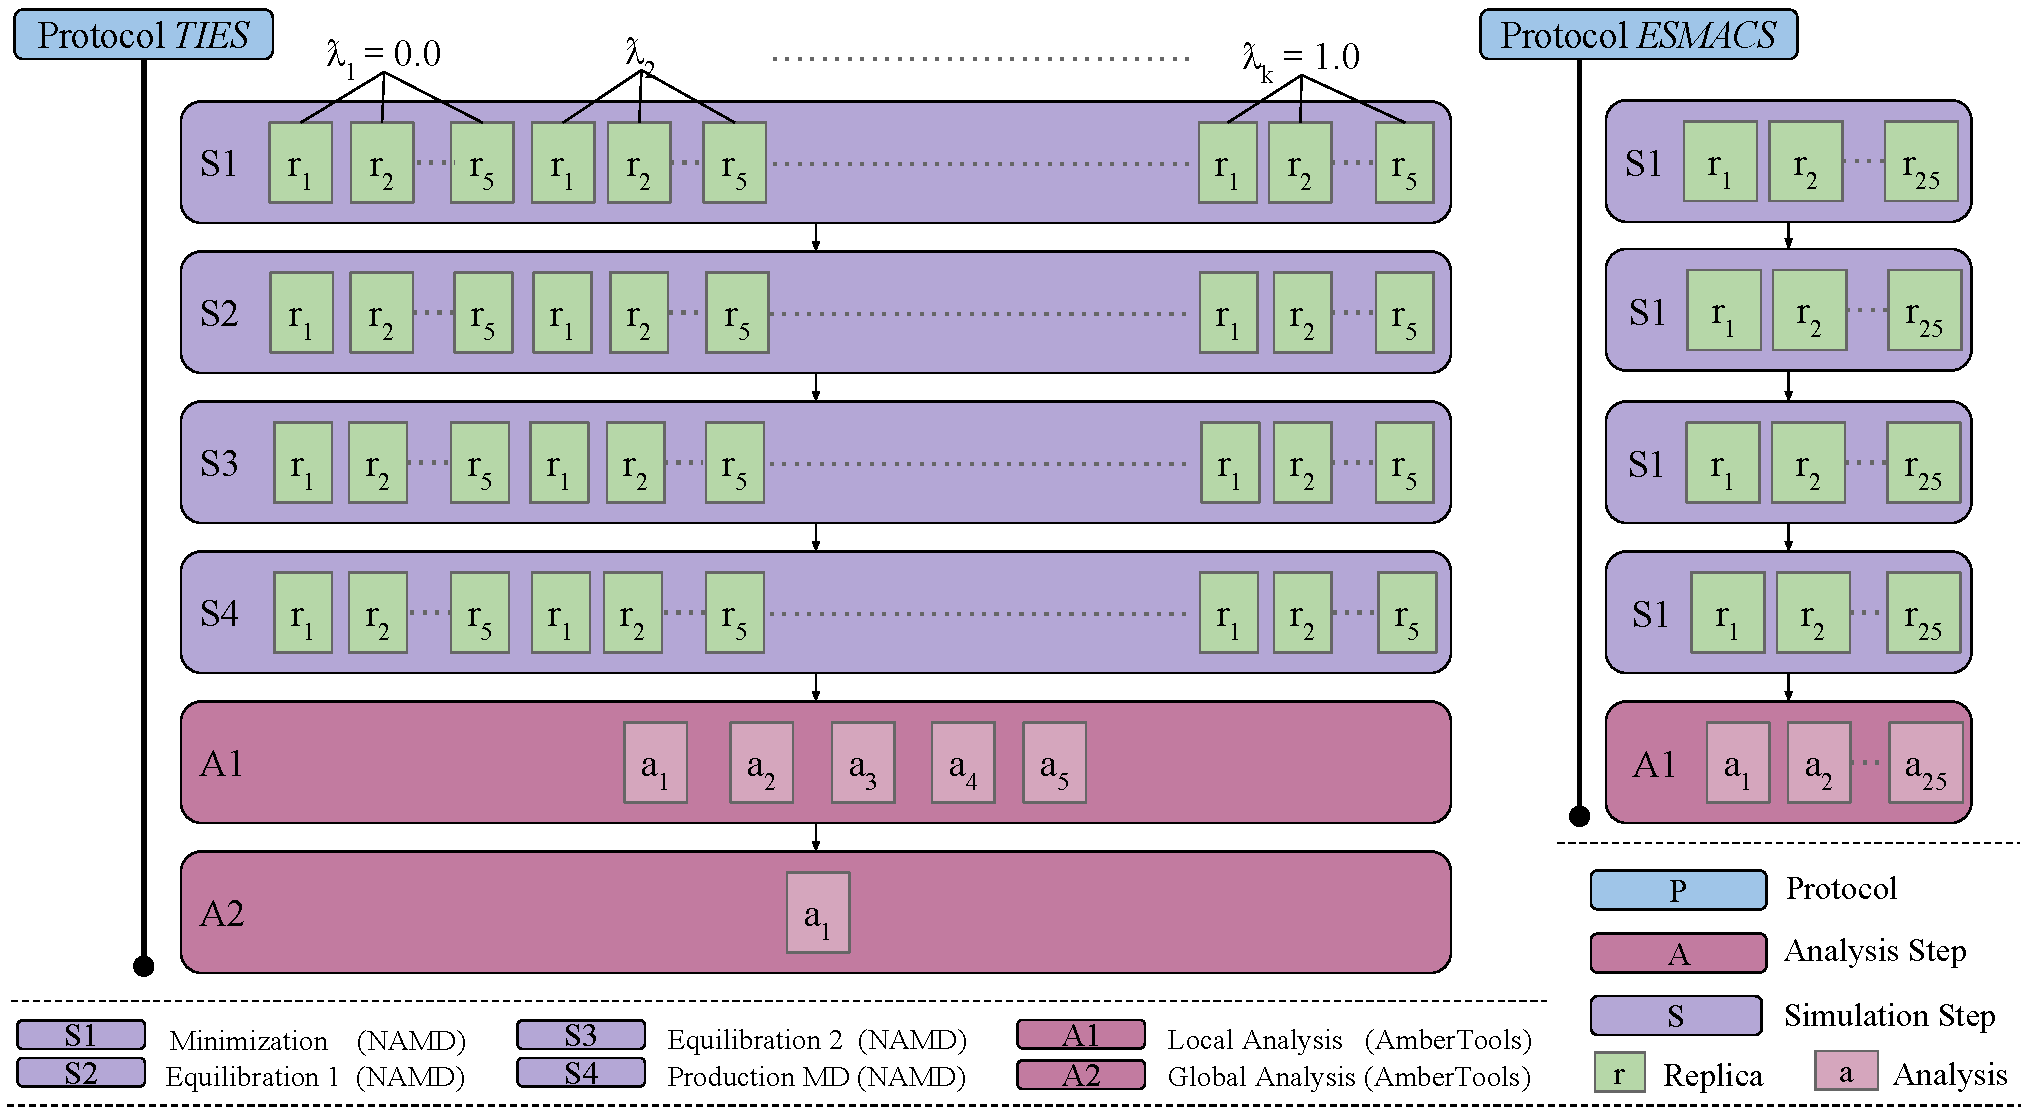
\includegraphics[width=\linewidth]{figures/bio_workflow.pdf}
%        \caption{}
%        \label{fig:bio_workflow}
%    \end{subfigure}%
%    ~ 
%    \begin{subfigure}[b]{0.45\textwidth}
%        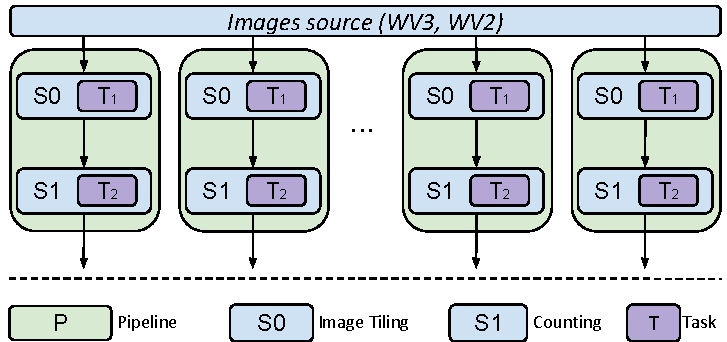
\includegraphics[width=\linewidth]{figures/earth_workflow.pdf}
%        \caption{}
%        \label{fig:earth_workflow}
%    \end{subfigure}
%    \caption{Biomolecular and Earth Science example workflows. \ref{fig:bio_workflow} Biomolecular workflow based on PST model example~\cite{dakka2018concurrent}; \ref{fig:earth_workflow} Earth science workflow based on PST model example~\cite{paraskevakos2019workflow}}\label{fig:bio_earth_workflows}
%\end{figure*}

%Computational campaigns resource requirements can be heterogeneous and cover a broad spectrum of resource types and numbers.
%Biomolecular science software tools support MPI/OpenMP, GPUs, and other accelerators, such as Intel Phi processors~\cite{cheatham2015impact} for executing either physical systems simulations or trajectory data analysis. \mtnote{simulations of? Analysis of?}
%In addition, some biomolecular analysis tool require specific computational environment or frameworks, such as Parallel MDAnalysis~\cite{fan2019pmda}, HiMach~\cite{tiankai2008scalable}.\mtnote{expand acronym, add other examples.}.
%Earth sciences applications, based on imagery, use workflows that execute a series of CPU based preprocessing, and eventually execute a computer vision algorithm on GPUs~\cite{paraskevakos2019workflow}\mtnote{This is specific to the applications you worked on, not necessarily true for all workflows used by the earth sciences communities. This comment seems to apply also to all the other examples of this paragraph}.


%The makespan of a campaign can be \mtnote{missing verb: derived maybe?} from a simple arithmetics calculation to a complex problem, depending on the heterogeneity of the campaign's workflows, maximum concurrency and resource dynamicity. \mtnote{This seems to assume that the reader has to understand the relation between makespan, heterogeneity and dynamicity on her own. I would refine and explain better.}
%Workflows can be heterogeneous in space, i.e., the number of tasks and resource requirements, and in time, i.e., the execution time needed to execute.
%When workflows are the same in space and time, they are considered homogeneous.
%Assuming enough resources to execute a workflow, when a campaign consists of homogeneous workflows any order of workflow execution would provide the same makespan. 
%When heterogeneity is introduced, randomly ordering the workflows' execution provides different makespan for different instances of the ordering.
%This is especially true, when there are not enough resources to execute all the workflows concurrently.
%As a result, calculating the makespan of the campaign based on workflow order execution becomes important to decide whether the selected mapping satisfies or not the campaign's computational campaign \mtnote{``campaign's computational campaign'' makes no sense.}.

\mtnote{This seems to assume that the reader has to understand the relation between makespan, heterogeneity and dynamicity on her own. I would refine and explain better.}\gpnote{Broke it into two paragraphs.}
Several factor can influence the complexity of calculating the makespan of a campaign, such as heterogeneity of the campaign's workflows, concurrency and resource dynamicity.
Workflows can be heterogeneous in space, i.e., the number of tasks and resource requirements, and in time, i.e., the execution time needed to execute.
When workflows are the same in space and time, they are considered homogeneous.
Assuming homogeneous workflows and a single static resource, the makespan of the campaign is equal to the addition of the execution time of all workflows.
When workflows from the campaign can be executed concurrently on static resources, the makespan of the campaign is equal to rounding up the division of the number of workflows to the number of resources times the execution time of a single workflow.
Dynamic resources can influence the makespan, since they will affect the maximum number of workflows that were executed serially in a resource.
As a result, any order of executing the workflows of a campaign produces the same makespan, which also is the minimum makespan.

When workflows are heterogeneous, the level of concurrency, resource dynamicity, and workflow execution order can affect the makespan.
In the case of sequential execution of the workflows, the order of the execution does not affect the makespan of the campaign.
When concurrency is introduced, the order and placing of workflows can affect the makespan of the campaign.
For example, a campaign has 9 heterogeneous in time workflows with sorted execution times from 1 to 9 time units, and they can be executed on three resources.
A possible execution order would be to place three consecutive workflows to each resource.
The makespan would be equal to the summation of the execution time of last workflows, i.e. $7 + 8 + 9 = 24$ time units.
Instead, executing the three workflows with the largest concurrently and position new workflows to resources as they become available, it can produce a makespan of $16$ time units.
This problem becomes complicated when the number of workflows in the campaign is in the order of thousands.



% ----------------------------------------------------------------------------
% campaign makespan modeling
We propose to initially utilize and extend the Heterogeneous Earliest Finish Time (HEFT)~\cite{topcuoglu2002performance} algorithm to calculate the makespan of computational campaigns\mtnote{for doing what?}.
HEFT is an offline scheduling algorithm which calculates the makespan of a workflow on heterogeneous resources, in terms of performance.
HEFT makes two important assumptions.
First, any task in a workflow can be executed in all available resources, and second all resources are always available.
HEFT is mainly used to derive and execution plan for workflows, i.e. the execution order and resource placement of the tasks that comprise the workflow.
Because we are interested in campaigns, our HEFT extension will provide an execution plan based on workflows as the unit it will operate.
HEFT uses a matrix to represent execution time of tasks on resources, assigning tasks to the resource that minimizes the finish time of the task, and has complexity proportional to the number of dependencies between tasks and the number of resources offered.\mtnote{Why suddenly are we writing about tasks? What is the relationship between HEFT, tasks, workflows and campaigns?}
Furthermore, there has been some initial research to extend HEFT to resources that provide CPU and GPUs~\cite{shetti2013optimization}, as well as a HEFT extension on dynamic resources~\cite{dong2007pfas}.

We identify four points of possible extensions:
\begin{inparaenum}[(i)]
    \item some workflows may not fit some resources,
    \item resources are becoming unavailable during execution,
    \item user may want some workflows to have higher priority than others, and
    \item multiple workflows may fit in a single resource.
\end{inparaenum}
Because workflows are heterogeneous in space and time, we assume that at least one resource can satisfy the computational requirements of every workflow, but not necessarily all resources.
Resources may become unavailable because the user has no allocation left, a scheduled maintenance is taking place, or some unscheduled downtime.
During the execution of a campaign, some workflows may have a higher priority compared to other due to user preference, or as response to an unforeseen event.
As a result, HEFT's data structure and HEFT needs to be extended to identify whether a workflow can be executed in a given resource or not, whether a resource is available or not, and user provided initial priorities.
Finally, a resource may be large enough so that multiple workflows may be able to execute concurrently.
We will investigate how HEFT can be extended to support variable resource capacity.\gpnote{It may need further extension.}

%There are several alternative methods and algorithms to calculate and optimize the makespan of a workflow~\cite{lu2019review}, including queuing networks~\cite{yao2019throughput,bao2019performance}, domain specific languages~\cite{carothers2017durango,maheshwari2016workflow}, and machine learning~\cite{witt2019predictive,pumma2017runtime}.
%Queuing networks will be of limited use because they require from the user to provide a queuing network equivalent of the campaign.
%As a result, having the user provide a queuing network representation of the campaign adds an additional layer of complexity. \mtnote{These two sentences are unclear, please revise.}
%Domain specific languages would require too much engineering effort to convert a workflow representation based on domain specific assumptions, e.g., MPI style workflow, or specific languages representation, e.g., Swift, to a PST model representation \mtnote{This is unconvincing: we choose to use the PST model and then we say that it requires too much effort? Remember: the argumentation here has to be `scientific', not just based on 'I want to use EnTK so this would require too much time'.}.
%Machine Learning approaches would require model training, validation and testing to produce a model \mtnote{Why would this be a problem?}.
%In addition, since the execution is done on dynamic resources, the model should be retrained after every workflow execution.

There are several alternative methods and algorithms to calculate and optimize the makespan of a workflow~\cite{lu2019review}, including queuing networks~\cite{yao2019throughput,bao2019performance}, domain specific languages~\cite{carothers2017durango,maheshwari2016workflow}, and machine learning~\cite{witt2019predictive,pumma2017runtime}.
Queuing networks will be of limited use because they require from the user to provide a queuing network equivalent to the campaign.
In the case the campaign contains only independent workflows, a single queue system with multiple servers would be sufficient, but a campaign with complex dependencies between workflows may require expertise outside of the user domain to define the equivalent queuing network.
HEFT sorts workflows based on the number of dependencies they have in the campaign.
\mtnote{These two sentences are unclear, please revise.}\gpnote{any better?}
% Application models contain descriptions of resource usage of an algorithm (such as the computation and communication require- ments) and control flow (iteration, sequential and parallel dependencies, and kernel nesting).
Domain specific languages approaches either require description of the resource usage of workflows~\cite{carothers2017durango}, or execute part of the campaign to obtain execution skeleton of the campaign~\cite{maheshwari2016workflow}.
When executing a campaign, workflows may require days to execute to obtain execution time information, and users rarely know the resource usage of their workflows to provide enough useful information.
In addition, the workflow of a campaign may be different and executing some of them may not provide any information about the execution of others.
\mtnote{This is unconvincing: we choose to use the PST model and then we say that it requires too much effort? Remember: the argumentation here has to be `scientific', not just based on 'I want to use EnTK so this would require too much time'.}
Similarly, machine learning approaches would be of limited use since there is no guarantee that the workflows of a campaign is are going to be similar.
As a result, to gather enough information to build a makespan calculation model may require the execution of the campaign.\mtnote{Why would this be a problem?}\gpnote{changed it}.
We want to provide an approach that only requires the user to provide as few information as possible, such as the workflows and an educated guess of their execution time  \gpnote{any better?}.


% ----------------------------------------------------------------------------
% Initial Assumptions
%We propose to extend HEFT to support execution of a computational campaign on dynamic resources \mtnote{and heterogeneous?}.
%When executing a workflows HEFT assumes that any available resource can execute the workflow's tasks \mtnote{Why this statement is relevant?}.
%In addition, when executing a workflow on HPC resources, it can be assumed that all the resources will be available during the execution of the workflows \mtnote{Explain further, you seem to be assuming the reader understand a lot of implications of what you are writing. This is generally untrue has the reader has a very different background from yours and never thought to what you are writing here before.}.
%These two assumptions are not necessarily true when a computational campaign is executed.
%As campaign's workflows are heterogeneous, not all resources will satisfy the space requirements for all the workflows \mtnote{why?}.
%Introducing resource dynamicity requires HEFT to take into account resource availability to decide on which resources it will schedule workflows.
%In addition, it should update the schedule as resources become unavailable.

% ----------------------------------------------------------------------------
% Campaign Manager definition, requirements, features and capabilities
We propose to design a campaign manager (CM) which, given a campaign, an objective, and a set of constraints, can derive an execution plan by utilizing the proposed makespan HEFT method, and execute a campaign.
If necessary the CM will change the execution plan by updating workflow to resource mapping, and resource availability.
Execution planning for workflows are provided by several workflow execution systems, such as Pegasus~\cite{deelman2015pegasus}, and ASKALON~\cite{fahringer2005askalon}.
Campaign management systems, such as PanDA~\cite{maeno2008panda}, do not provide a campaign planning feature.
QCFractal~\cite{qcfractal} offers some form of planning by allowing user to specify the priority of a workflow in a campaign, but it does not plan with taking into account the makespan of the campaign.\mtnote{only these two among all the existing systems? Please refine and expand, explaining that these are just examples. Also, expand appropriately introducing the notions of planning and plan and explaining why they relate to campaign management.}\gpnote{I introduced the plan a few paragraphs before. It may still need to be expanded.}


Figure~\ref{fig:refarch} shows a reference architecture where the CM has three components:
\begin{inparaenum}[(1)]
\item a Planner,
\item and Enactor, and
\item a Bookkeeper. 
\end{inparaenum}
Workflow execution will be done through an existing workflow management framework (WMF) on HPC resources.
Plan updates will be based on workflows execution metrics provided by the selected WMF such as tasks execution time, overheads calculation and time to completion.
These metrics will be aggregated across workflows resulting in campaign-wide execution metrics.

\begin{figure*}[t]
    \centering
    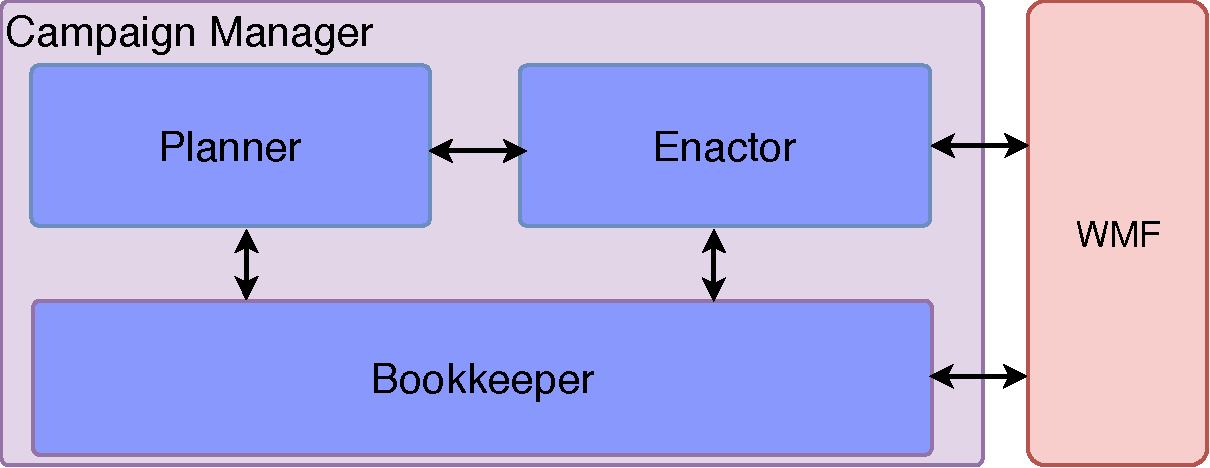
\includegraphics[width=.95\textwidth]{figures/CEM_design.pdf}
    \caption{Reference Architecture of a Campaign Manager. Basic 
    components of Campaign Manager (CM): 1) Planner, 2) Enactor and 3) Bookkeeper. 
    CM communicates decisions to RADICAL-EnTK. CM communicates with HPCs to 
    execute parts of the campaign.}\label{fig:refarch}
\end{figure*}

The Planner will be responsible for deriving an execution plan  \mtnote{is it a calculator or an optimizer? Seem different capabilities to me and not necessarely part of the same component} the makespan of a campaign based on a set of resources, and the objective.
It will utilize the extend HEFT algorithm to derive an execution plan of the campaign. \mtnote{It seems to me that makespan calculation is only one of the elements needed to derive a plan. As such, I think you need at least two components in your architecture: makespan calculator and planner.}
In addition based on information from the other components, the planner may update the plan accordingly.

The Bookkeeper component is responsible to monitor the execution of the campaign.
This component knows the state of the campaign, the execution plan, the availability of the resources, and the campaign's objective.
The state of the campaign is based on information that the bookkeeper is receiving from the used WMF and the enactor component.
In addition, it knows the state of the resources, the campaign is using.
Based on this set of information, it checks whether the campaign's objective can be achieved.
If any change in the campaign happens, such as workflows are added or removed, a resource is not available any more, or the objective is not going to be met, the bookkeeper informs the planner to update the plan.
An important feature of the bookkeeper is to identify the reason of a failing workflow.
When the failure is because the resource is not available, the specific workflow may need to be executed and the plan to be updated.

The Enactor is responsible to execute the plan decided by the planner by interfacing with the WMF.
Based on the plan, the enactor is responsible to execute workflows on the respective resources based on the plan.
To achieve that, the enactor informs the WMF to acquire resources, translates the workflow from the user's specification to the API provided by the WMF, and submits the workflow.
In the case where a group of workflows is to be executed as a single workflow, the enactor is responsible to group them as well.
Furthermore, it informs the bookkeeper which workflows were submitted for execution.

%The Executor sub-component is responsible to execute and monitor the plan \mtnote{where is the plan coming from?} by interfacing with a WMF.
%Based on the plan the Makespan calculator decided, the Executor submits workflows to a WMF to execute on the selected resource.
%This requires the Executor to work upon multiple workflows concurrently \mtnote{and why is this important?}.
%In addition, it should monitor workflow execution and resource availability \mtnote{why?}.
%An important requirement for the executor is to identify the reason of a failing workflow.
%When the failure is because the resource is not available, the specific workflow may need to be rescheduled and the plan to be updated.

RADICAL-Ensemble Toolkit~\cite{balasubramanian2018harnessing} (EnTK) is a workflow management framework.
We selected to utilize EnTK because it fits the requirements of the target use cases, and it utilizes a pilot framework as its runtime system.
EnTK defines workflows as a set of pipelines, each pipeline is a sequence of stages, and in turn each stage a set of tasks.
Concurrency during execution happens at the level of pipelines and tasks.
Furthermore, EnTK supports the execution of a sequence of workflows by either reusing already acquired resources or by requesting new ones\mtnote{grammar: from `may' onwards I do not understand the sentence anymore.}.
EnTK workflow execution is stateful, provides execution timing traces for tasks and workflows, and supports workflow execution on multiple HPC resources.
Furthermore, EnTK utilizes a pilot runtime system, RADICAL-Pilot~\cite{merzky2019using}, to execute workflows on HPC resources.
Pilot systems submit job placeholders on resources, and are able to execute tasks on the acquired resources.
This capability allows to execute multiple workflows to resources that are acquired once, either sequentially or concurrently.
%As a result, the campaign manager will see a set of resources where workflows should be executed upon \mtnote{not sure  understand how this follows from your explanation of pilots.}.
The proposed campaign manager will interface with EnTK through the enactor and bookkeeper components to execute and monitor workflows based on the derived execution plan.

\mtnote{General note: this needs to be expanded following the comments I left. At the moment, a lot of this still reads as a set of sometimes disconnected statements. We need to iterate so to produced a more detailed description of the research you propose to conduct in the next year, a description backed by existing literature and your own argumentation. From our discussions, I know you have the material needed to iterate this initial draft.}
